\section{Kinematik, Kräfte \& Dynamik}
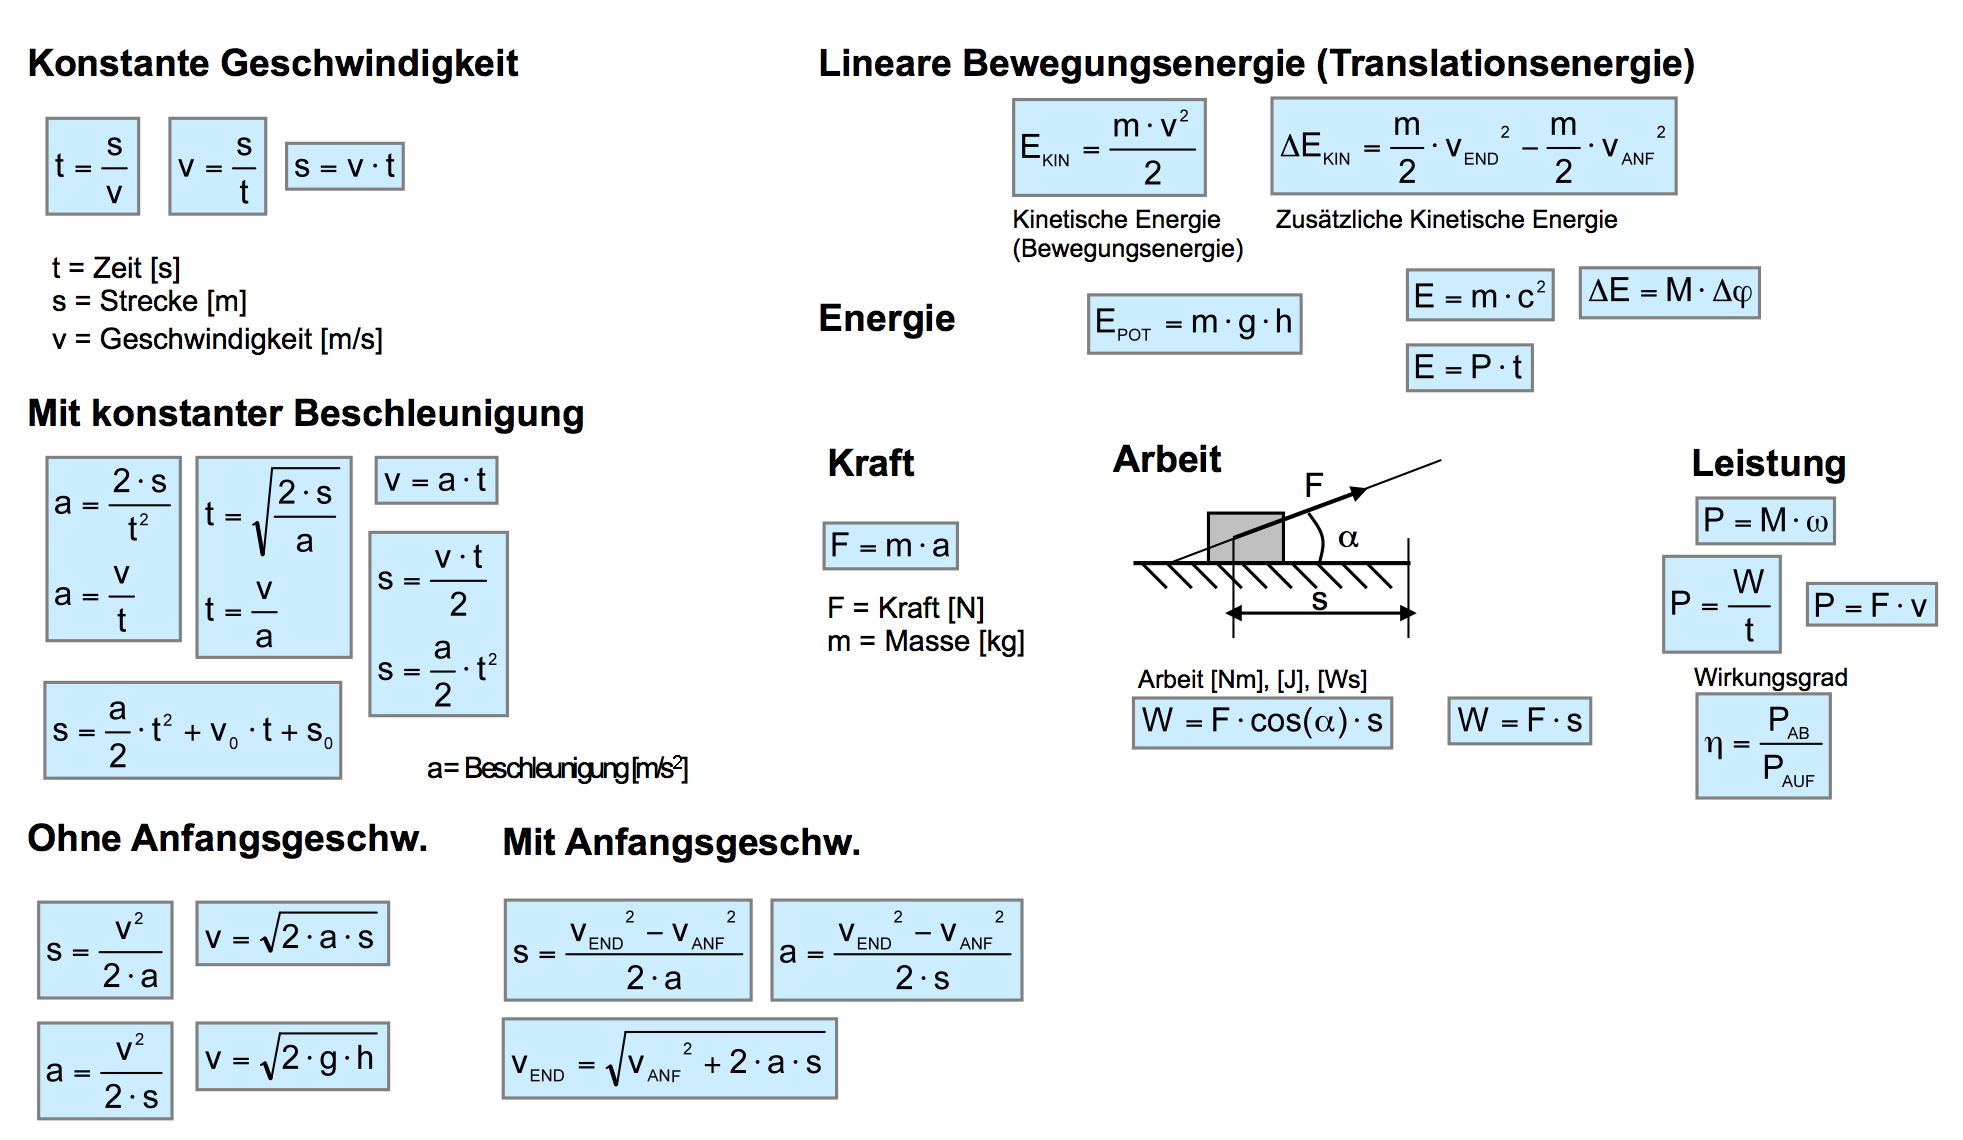
\includegraphics[width=17cm]{./bilder/kinematik.png} \\

\subsection{Kräfte}
$\tau_{n}={}^0J^T_n \cdot {}^0F_n  \\ \\
{}^0F_n = \begin{bmatrix} {}^0F_{x,n} & {}^0F_{y,n} & {}^0F_{z,n} & {}^0M_{x,n}
& {}^0M_{y,n} & {}^0M_{z,n}
\end{bmatrix}^{T}  \\ \\
zum Beispiel: \\
\begin{bmatrix}
\tau_{1} \\ \tau_{2} \\ \tau_{3}
\end{bmatrix}          
=  J \cdot
\begin{bmatrix}
F_{x} \\ F_{y} \\ F_{z}
\end{bmatrix}
$